\chapter{पश्च-संश्लेषण और बहुचरणीय रणनीति}\label{ch:b2:retrosynthesis}

बोर्ड पर एक अणु बनाया गया है, और अभी कोई नहीं जानता कि उसे कैसे बनाया जाए। जो कुछ ताक पर है, उससे
अभिक्रियाओं को आगे की ओर आज़माना कहीं नहीं ले जाता: वे बहुत अधिक हैं। रसायनज्ञ उलटी दिशा में काम करता है,
लक्ष्य से पीछे ताक की ओर, काग़ज़ पर एक बार में एक आबंध काटते हुए, हर कटाव किसी ऐसी अभिक्रिया को उलटता है
जिसका काम करना ज्ञात है, जब तक कि टुकड़े ऐसे यौगिक न हो जाएँ जो ख़रीदे जा सकें। यह अध्याय
पिछले अध्यायों की अभिक्रियाओं को उस पीछे की ओर के तर्क में बदलता है, और फिर पूछता है कि उससे बने मार्ग को कैसे परखा जाए।

\begin{recall}
\Cref{ch:b2:alkene-redox} से \cref{ch:b2:wittig} तक: उलटी जाने वाली अभिक्रियाएँ। प्रथम वर्ष का खंड:
रक्षी समूह और ऐसीटैल, ग्रीन्यार अभिकर्मक और ध्रुवता प्रतिलोमन, विलियमसन संश्लेषण,
रसायनवरणात्मकता, ऐल्कोहॉलों का ऑक्सीकरण। विद्यालय का खंड: परमाणु मितव्ययिता।
\end{recall}

\section{पीछे की ओर सोचना}

\begin{definition}[पश्च-संश्लेषी विश्लेषण]\label{def:b2:retrosynthesis:analysis}
जिस अणु को बनाना है वह \emph{लक्ष्य अणु}\index{लक्ष्य अणु} है। \emph{पश्च-संश्लेषी विश्लेषण}
\index{पश्च-संश्लेषी विश्लेषण} लक्ष्य से पीछे उपलब्ध आरंभिक पदार्थों की ओर काम करता है,
ऐसे चरणों द्वारा जिनमें से हर एक किसी ज्ञात अभिक्रिया का उलटा है; पश्च-संश्लेषी चरण
द्वि-तीर $\Rightarrow$ से लिखा जाता है, और ``से बनता है'' पढ़ा जाता है।
\end{definition}

\begin{definition}[विच्छेदन और सिंथॉन]\label{def:b2:retrosynthesis:disconnection}
\emph{विच्छेदन}\index{विच्छेदन} लक्ष्य के किसी आबंध का काल्पनिक कटाव है, जो आबंध बनाने वाली किसी अभिक्रिया का
उलटा है। किसी आबंध को विषमांशी रूप से काटने पर दो \emph{सिंथॉन}\index{सिंथॉन} मिलते हैं,
आदर्शीकृत आवेशित खंड, एक दाता (नाभिकरागी, प्रायः ऋणात्मक), दूसरा ग्राही
(इलेक्ट्रॉनरागी, प्रायः धनात्मक)। \emph{संश्लेषी तुल्य}\index{संश्लेषी तुल्य} कोई वास्तविक
अभिकर्मक है जो सिंथॉन की तरह व्यवहार करता है: कार्बऋणायन \ce{R-} के लिए ग्रीन्यार अभिकर्मक,
धनायन $\mathrm{R\overset{+}{C}H{-}OH}$ के लिए ऐल्डिहाइड।
\end{definition}

\begin{definition}[क्रियात्मक-समूह अंतर्रूपांतरण]\label{def:b2:retrosynthesis:fgi}
\emph{क्रियात्मक-समूह अंतर्रूपांतरण}\index{क्रियात्मक-समूह अंतर्रूपांतरण} (FGI) वह
पश्च-संश्लेषी चरण है जो कार्बन ढाँचे को बदले बिना किसी क्रियात्मक समूह को बदलता है: ऐल्कोहॉल
कीटोन से (अपचयन द्वारा), ऐल्केन शृंखला ऐल्कीन से (हाइड्रोजनन द्वारा), ऐमीन ऐमाइड से।
\end{definition}

\begin{omfigure}
\begin{tikzpicture}[every node/.style={align=center}]
\node (T) at (0,0) {\setchemfig{atom sep=1.7em}\chemfig{Ph-CH(-[2]OH)-CH(-[6]CH_3)-CH_3}};
\node (A) at (-4.6,-2.6) {\ce{PhCHO}\\[1pt] + \ce{(CH3)2CHMgBr}};
\node (B) at (0,-2.6) {\ce{PhMgBr}\\[1pt] + \ce{(CH3)2CHCHO}};
\node (C) at (4.6,-2.6) {\setchemfig{atom sep=1.7em}\chemfig{Ph-C(=[2]O)-CH(-[6]CH_3)-CH_3}};
\node (D) at (4.6,-5.0) {\ce{C6H6}\\[1pt] + \ce{(CH3)2CHCOCl}};
\draw[omretro] (T.south west) -- node[above left, font=\small] {a} (A.north);
\draw[omretro] (T.south) -- node[right, font=\small] {b} (B.north);
\draw[omretro] (T.south east) -- node[above right, font=\small] {FGI} (C.north);
\draw[omretro] (C.south) -- node[right, font=\small] {c} (D.north);
\end{tikzpicture}
\par\vspace{6pt}

{\small 2-मेथिल-1-फ़ेनिलप्रोपेन-1-ऑल का एक पश्च-संश्लेषी वृक्ष। (a) और (b): ऐल्कोहॉल कार्बन के बगल वाले
\ce{C-C} आबंध के दोनों \omterm{def:b2:retrosynthesis:disconnection}{विच्छेदन}, हर एक में एक ऐल्डिहाइड और एक ग्रीन्यार अभिकर्मक। FGI: ऐल्कोहॉल
कीटोन से, अपचयन द्वारा; (c) बेन्ज़ीन के \omterm{def:b2:aromatic-substitution:friedel-crafts}{फ़्रीडेल--क्राफ़्ट्स ऐसिलन} से कीटोन। हर तीर
``से बनता है'' पढ़ा जाता है।}
\end{omfigure}

वृक्ष विधि की आदतें दिखाता है। \omterm{def:b2:retrosynthesis:disconnection}{विच्छेदन} किसी क्रियात्मक समूह के बगल वाले आबंध पर चुना जाता है,
क्योंकि अभिक्रियाएँ वहीं आबंध बनाती हैं। हर कटाव की जाँच \omterm{def:b2:retrosynthesis:disconnection}{सिंथॉन} लिखकर और उनके लिए
वास्तविक अभिकर्मक खोजकर की जाती है। और उत्तर शायद ही कभी एक होता है: वृक्ष शाखित होता है, और शाखाओं को
अंत में परखा जाता है (\cref{sec:b2:retrosynthesis:judging})।

\begin{omfigure}
\begin{center}
\small
\renewcommand{\arraystretch}{1.25}
\begin{tabular}{lll}
\hline
\omterm{def:b2:retrosynthesis:disconnection}{सिंथॉन} & प्रकार & \omterm{def:b2:retrosynthesis:disconnection}{संश्लेषी तुल्य} \\
\hline
\ce{R-} (ऐल्किल, ऐरिल) & दाता & \ce{RMgBr}, \ce{RLi}, \ce{R2CuLi} (संयुग्मी) \\
$\mathrm{^-CH_2COR}$ & दाता & \ce{CH3COR} का \omterm{def:b2:enolates-aldol:enolate}{ईनोलेट}, या एथिल 3-ऑक्सोब्यूटेनोएट \\
$\mathrm{^-C{\equiv}N}$ & दाता & \ce{NaCN} \\
$\mathrm{R\overset{+}{C}H{-}OH}$ & ग्राही & ऐल्डिहाइड \ce{RCHO} \\
$\mathrm{R\overset{+}{C}{=}O}$ & ग्राही & \omterm{def:b2:acyl-substitution:derivative}{ऐसिल क्लोराइड} \ce{RCOCl}, कोई एस्टर \\
\ce{R+} (प्राथमिक) & ग्राही & हैलाइड \ce{RBr} (द्वि-अणुक प्रतिस्थापन) \\
$\mathrm{^+CH_2CH_2COR}$ & ग्राही & ईनोन \ce{CH2=CHCOR} (\omterm{def:b2:conjugate-additions:addition-modes}{संयुग्मी योग}) \\
\hline
\end{tabular}
\end{center}

{\small सामान्य \omterm{def:b2:retrosynthesis:disconnection}{सिंथॉन} और उनके \omterm{def:b2:retrosynthesis:disconnection}{संश्लेषी तुल्य}। दाता \omterm{def:b2:retrosynthesis:disconnection}{सिंथॉन} कार्बऋणायन हैं,
ग्राही \omterm{def:b2:retrosynthesis:disconnection}{सिंथॉन} कार्बधनायन; वास्तविक अभिकर्मक पूर्ण आवेश के बिना वही ध्रुवता रखते हैं।}
\end{omfigure}

\section{एक-समूह विच्छेदन}

एक-समूह \omterm{def:b2:retrosynthesis:disconnection}{विच्छेदन} किसी अकेले क्रियात्मक समूह के बगल वाले आबंध को काटता है। किसी ईथर, एस्टर या ऐमीन के
\ce{C-O} या \ce{C-N} आबंध के लिए कटाव कार्बन और विषमपरमाणु के बीच जाता है: विषमपरमाणु
दाता है, कार्बन ग्राही (विलियमसन संश्लेषण, \omterm{def:b2:acyl-substitution:esterification}{एस्टरीकरण}, ऐमाइड का बनना)।
\ce{C-C} आबंध के लिए क्रियात्मक समूह \omterm{def:b2:retrosynthesis:disconnection}{सिंथॉनों} की ध्रुवता तय करता है: किसी ऐल्कोहॉल कार्बन के बगल में
ऐल्कोहॉल कार्बन ग्राही है (कोई ऐल्डिहाइड या कीटोन) और दूसरा कार्बन दाता (कोई
कार्बधात्विक यौगिक); किसी कार्बोनिल के बगल में $\alpha$ कार्बन दाता है (एक \omterm{def:b2:enolates-aldol:enolate}{ईनोलेट})।

इनमें से अधिकांश अभिक्रियाओं को सही स्थान पर सही ऑक्सीकरण स्तर चाहिए, अतः ऑक्सीकरण
स्तरों के बीच FGI किसी मार्ग के सबसे सामान्य चरण हैं: ऐल्कीन, ऐल्कोहॉल, ऐल्डिहाइड या कीटोन, अम्ल। इनमें से एक
प्रथम वर्ष के खंड में खुला छोड़ा गया था: किसी प्राथमिक ऐल्कोहॉल के ऑक्सीकरण को ऐल्डिहाइड पर रोकना।

\begin{proposition}[मृदु ऑक्सीकरण]\label{prop:b2:retrosynthesis:mild-oxidation}
किसी निर्जल कार्बनिक विलायक में प्रयुक्त ऑक्सीकारक से प्राथमिक ऐल्कोहॉल, अम्ल तक गए बिना,
ऐल्डिहाइड तक ऑक्सीकृत होता है: डाइक्लोरोमेथेन में पिरिडीनियम क्लोरोक्रोमेट, स्वर्न ऑक्सीकरण (ऑक्सैलिल क्लोराइड से
सक्रियित डाइमेथिल सल्फ़ॉक्साइड, फिर ट्राइएथिलऐमीन, निम्न ताप पर) या डेस--मार्टिन
पीरियोडिनेन। जल में क्रोमियम(VI) या परमैंगनेट उसे कार्बोक्सिलिक अम्ल तक ऑक्सीकृत करते हैं।
\end{proposition}

\begin{proof}[तर्क]
ये ऑक्सीकारक \ce{C-H} आबंध का हाइड्रोजन हटाते हैं, उस कार्बन पर जो \ce{OH} धारण करता है। बने ऐल्डिहाइड
में ऐसा कोई समूह नहीं है। परंतु जल में कोई ऐल्डिहाइड अपने जलयोजित रूप
\ce{RCH(OH)2} के साथ साम्य में होता है, जिसमें फिर से हाइड्रोजन धारण करने वाले कार्बन पर \ce{OH} है: जलयोजित रूप
ऐल्कोहॉल की तरह, अम्ल तक, ऑक्सीकृत होता है। जल के बिना कोई जलयोजित रूप नहीं बनता, और ऑक्सीकरण
ऐल्डिहाइड पर रुक जाता है।
\end{proof}

\section{द्वि-समूह विच्छेदन}

जब लक्ष्य में दो क्रियात्मक समूह हों, तो सबसे अच्छा \omterm{def:b2:retrosynthesis:disconnection}{विच्छेदन} प्रायः दोनों का उपयोग करता है: आबंध ऐसे काटा जाता है
कि एक समूह दाता को निर्देशित करे और दूसरा ग्राही को। समूहों के बीच की दूरी,
एक क्रियाशील कार्बन से दूसरे तक दोनों को सम्मिलित करते हुए कार्बनों में गिनी गई, बताती है कि कौन-सी अभिक्रिया प्रयुक्त की जाए।

\begin{proposition}[पैटर्न और उनकी अभिक्रियाएँ]\label{prop:b2:retrosynthesis:patterns}
दो समूहों के बीच के संबंध पिछले अध्यायों की अभिक्रियाओं से इस प्रकार मेल खाते हैं।
विषम संबंध (1,3 और 1,5) कार्बोनिल रसायन की स्वाभाविक ध्रुवताओं से मेल खाते हैं; सम संबंध (1,4
और 1,6) नहीं, और उन्हें ध्रुवता प्रतिलोमन या किसी वलय के विदलन की आवश्यकता होती है।
\end{proposition}


\begin{proof}[तर्क]
कार्बोनिल रसायन में कार्बोनिल कार्बन ग्राही है और $\alpha$ कार्बन दाता, और कोई ईनोन
अपने $\beta$ कार्बन पर एक ग्राही जोड़ता है। किसी कार्बोनिल (कार्बोनिल कार्बन पर ग्राही) पर कोई \omterm{def:b2:enolates-aldol:enolate}{ईनोलेट} ($\alpha$ पर दाता)
1,3 पैटर्न के कार्बन 1 और 2 को जोड़ता है: \omterm{def:b2:enolates-aldol:aldol}{ऐल्डोल} और क्लाइज़न। किसी ईनोन के $\beta$
कार्बन पर \omterm{def:b2:enolates-aldol:enolate}{ईनोलेट} 1,5 पैटर्न बनाता है: माइकल, फिर रॉबिन्सन। 1,4 पैटर्न के लिए कटाव एक
$\alpha$ कार्बन को ग्राही के रूप में छोड़ता है; कोई सामान्य कार्बोनिल अभिकर्मक वह ध्रुवता नहीं देता, परंतु कोई $\alpha$-ब्रोमो
कीटोन देता है, क्योंकि उस कार्बन पर ब्रोमाइड निर्गामी समूह है। 1,6 डाइकार्बोनिल \omterm{def:b2:alkene-redox:cleavage}{ओज़ोनी-अपघटन} से खोला गया
साइक्लोहेक्सीन है (\cref{prop:b2:alkene-redox:ozonolysis}), और साइक्लोहेक्सीन \omterm{def:b2:frontier-orbitals:diels-alder}{डील्स--ऐल्डर
अभिक्रिया} से बनती है (\cref{def:b2:frontier-orbitals:diels-alder})।
\end{proof}

\begin{omfigure}
\begin{center}
\small
\renewcommand{\arraystretch}{1.25}
\begin{tabular}{lll}
\hline
लक्ष्य में पैटर्न & \omterm{def:b2:retrosynthesis:disconnection}{विच्छेदन} & अभिक्रिया \\
\hline
$\beta$-हाइड्रॉक्सी कार्बोनिल (1,3) & $\alpha$--$\beta$ आबंध & \omterm{def:b2:enolates-aldol:aldol}{ऐल्डोल योग} \\
$\alpha,\beta$-असंतृप्त कार्बोनिल & \ce{C=C} & \omterm{def:b2:enolates-aldol:aldol}{ऐल्डोल संघनन} \\
1,3-डाइकार्बोनिल & C(O)--C$\alpha$ & \omterm{def:b2:enolates-aldol:claisen}{क्लाइज़न संघनन} \\
1,5-डाइकार्बोनिल & ग्राही का C$\alpha$--C$\beta$ & \omterm{def:b2:conjugate-additions:michael}{माइकल योग} \\
साइक्लोहेक्स-2-ईन-1-ओन & वलय \ce{C=C}, फिर माइकल आबंध & \omterm{def:b2:conjugate-additions:robinson}{रॉबिन्सन वलयन} \\
साइक्लोहेक्सीन & वलय के दो \ce{C-C} आबंध & \omterm{def:b2:frontier-orbitals:diels-alder}{डील्स--ऐल्डर अभिक्रिया} \\
निर्धारित स्थान पर ऐल्कीन & \ce{C=C} & विटिग या HWE अभिक्रिया \\
1,4-डाइकार्बोनिल & केंद्रीय \ce{C-C} & \omterm{def:b2:enolates-aldol:enolate}{ईनोलेट} + $\alpha$-हैलो कीटोन \\
1,6-डाइकार्बोनिल & सिरों को फिर जोड़िए & साइक्लोहेक्सीन का \omterm{def:b2:alkene-redox:cleavage}{ऑक्सीकारी विदलन} \\
\hline
\end{tabular}
\end{center}

{\small द्वि-समूह \omterm{def:b2:retrosynthesis:disconnection}{विच्छेदन}। पहले छह सामान्य ध्रुवता का उपयोग करते हैं: किसी
कार्बोनिल या ईनोन (ग्राही) पर \omterm{def:b2:enolates-aldol:enolate}{ईनोलेट} (दाता)। 1,4 पैटर्न को चाहिए कि किसी कार्बोनिल के सापेक्ष $\alpha$ कार्बन
ग्राही हो, जो उसकी सामान्य भूमिका का उलटा है, और यह $\alpha$-हैलो कीटोन प्रदान करता है।}
\end{omfigure}

\begin{method}[पश्च-संश्लेषी विश्लेषण]\label{met:b2:retrosynthesis:retrosynthesis}
\begin{enumerate}
  \item लक्ष्य के क्रियात्मक समूहों और उनके संबंधों (1,2; 1,3; \dots) की सूची बनाइए।
  \item ऐसे FGI पर विचार कीजिए जो अच्छे \omterm{def:b2:retrosynthesis:disconnection}{विच्छेदन} वाला पैटर्न दें (कीटोन से ऐल्कोहॉल,
        ऐल्कीन से ऐल्केन शृंखला)।
  \item रणनीतिक आबंध चुनिए: किसी क्रियात्मक समूह के बगल में, अणु के मध्य के निकट, किसी
        शाखा-बिंदु पर या किसी वलय को शृंखला से जोड़ने वाले, ताकि टुकड़े समान आकार के हों।
  \item \omterm{def:b2:retrosynthesis:disconnection}{सिंथॉन} लिखिए, फिर उनके \omterm{def:b2:retrosynthesis:disconnection}{संश्लेषी तुल्य}; जिस कटाव का कोई वास्तविक अभिकर्मक न हो उसे अस्वीकार कीजिए।
  \item रसायनवरणात्मकता जाँचिए: हर अभिकर्मक से और कौन-सा समूह अभिक्रिया करेगा? किसी रक्षण की योजना बनाइए
        या चरणों का क्रम बदलिए।
  \item हर टुकड़े पर दोहराइए जब तक सभी उपलब्ध न हों; फिर अभिकर्मकों और
        परिस्थितियों के साथ मार्ग को आगे की ओर लिखिए।
\end{enumerate}
\end{method}

\section{किसी मार्ग में रक्षी समूह}

किसी मार्ग को प्रायः ऐसे अभिकर्मक की आवश्यकता होती है जो अणु के किसी दूसरे समूह पर आक्रमण कर देता। प्रथम वर्ष के खंड ने
ऐल्डिहाइडों और कीटोनों का ऐसीटैल के रूप में रक्षण किया था। कोई मार्ग कई रक्षी समूहों में से चुनता है, जिनमें से हर एक
अपनी परिस्थितियों से हटता है: ऐसीटैल (जलीय अम्ल से हटते हैं), ऐल्कोहॉलों के सिलिल ईथर (फ़्लुओराइड
आयन से हटते हैं), बेन्ज़िल ईथर (पैलेडियम पर हाइड्रोजन-अपघटन से हटते हैं), ऐमीनों के कार्बामेट जैसे
\textit{tert}-ब्यूटॉक्सीकार्बोनिल समूह (अम्ल से हटते हैं), और एस्टर (क्षारक से हटते हैं)।

\begin{definition}[लांबिक रक्षण]\label{def:b2:retrosynthesis:orthogonal}
\emph{लांबिक रक्षी समूहों}\index{लांबिक रक्षी समूह} का समुच्चय ऐसे रक्षी
समूहों का समुच्चय है जिनमें से हर एक ऐसी परिस्थितियों से हटाया जा सकता है जो बाक़ी सभी को अक्षत छोड़ देती हैं, ताकि उनके द्वारा ढकी
क्रियात्मकताएँ एक-एक करके, किसी भी क्रम में, मुक्त की जा सकें।
\end{definition}

\begin{method}[किसी मार्ग में रक्षण]\label{met:b2:retrosynthesis:protect-in-route}
\begin{enumerate}
  \item हर चरण के लिए उन समूहों की सूची बनाइए जिन पर अभिकर्मक इच्छित समूह के अतिरिक्त आक्रमण करेगा।
  \item पहले रक्षण से बचने का प्रयास कीजिए: चरणों का क्रम बदलिए, या अधिक वरणात्मक अभिकर्मक प्रयुक्त कीजिए
        (एस्टर के बगल वाले कीटोन के लिए हाइड्राइड के बजाय बोरोहाइड्राइड)।
  \item अन्यथा ऐसा समूह चुनिए जो हटाए जाने तक हर चरण में स्थायी रहे, और ऐसी परिस्थितियों में हटाया जा सके जिन्हें
        अणु सह सके।
  \item अलग-अलग मुक्त करने के लिए कई समूह हों, तो एक लांबिक समुच्चय चुनिए।
  \item ऐसा चरण खोजिए जो कोई समूह मुफ़्त में हटा दे: वैसे भी नियोजित हाइड्रोजनन किसी
        बेन्ज़िल ईथर को भी हटा देता है।
  \item गिनिए: हर रक्षण की क़ीमत दो चरण और उनकी लब्धियाँ हैं।
\end{enumerate}
\end{method}

\section{किसी मार्ग को परखना}\label{sec:b2:retrosynthesis:judging}

\begin{proposition}[समग्र लब्धि]\label{prop:b2:retrosynthesis:overall-yield}
चरणों के किसी रैखिक अनुक्रम की समग्र लब्धि चरण लब्धियों का गुणनफल है:
$\rho = \rho_1 \rho_2 \cdots \rho_n$। $n$ चरणों के साथ, जिनकी समान लब्धि $\rho_1$ हो, $\rho = \rho_1^{\,n}$।
\end{proposition}

\begin{proof}
चरण $k$ अपने आरंभिक पदार्थ की मात्रा $n_{k-1}$ को उत्पाद की मात्रा $n_k = \rho_k\, n_{k-1}$ में बदलता है
(लब्धियाँ मध्यवर्ती की मात्राओं पर ली गईं, अन्य सभी अभिकर्मक पर्याप्त मात्रा में)। आगमन से
$n_n = \rho_n \rho_{n-1} \cdots \rho_1\, n_0$, और समग्र लब्धि $n_n/n_0$ गुणनफल है।
\end{proof}

\begin{omfigure}
\begin{tikzpicture}
\begin{axis}[width=0.75\linewidth, height=5.4cm, xmin=0, xmax=20, ymin=0, ymax=100,
  xlabel={चरणों की संख्या $n$}, ylabel={समग्र लब्धि (\%)}, label style={font=\small},
  tick label style={font=\scriptsize}, xtick={0,5,10,15,20}, grid=major, grid style={black!12},
  legend style={font=\scriptsize, at={(0.98,0.98)}, anchor=north east}, legend cell align=left]
\addplot[omDef, thick] table[x=n, y=r95] {figdata/out/bachelor-2-overall-yield.dat};
\addplot[omThm, thick] table[x=n, y=r90] {figdata/out/bachelor-2-overall-yield.dat};
\addplot[omMeth, thick] table[x=n, y=r80] {figdata/out/bachelor-2-overall-yield.dat};
\addplot[black!60, thick, dashed] table[x=n, y=r70] {figdata/out/bachelor-2-overall-yield.dat};
\legend{95~\% प्रति चरण, 90~\% प्रति चरण, 80~\% प्रति चरण, 70~\% प्रति चरण}
\end{axis}
\end{tikzpicture}
\par\vspace{4pt}

{\small किसी रैखिक मार्ग की समग्र लब्धि उसके चरणों की संख्या के विरुद्ध, चार चरण लब्धियों के लिए
(\cref{prop:b2:retrosynthesis:overall-yield})। 90~\% के दस चरण पदार्थ का 35~\% बचाए रखते हैं; 70~\% के दस
चरण, 3~\% से कम।}
% figdata: bachelor-2/overall-yield.py
\end{omfigure}

गुणनफल नियम ही कारण है कि छोटे मार्ग जीतते हैं, कि कोई रक्षण (दो अतिरिक्त चरण) कभी मुफ़्त नहीं होता, और कि
रसायनज्ञ दो अर्धांश अलग-अलग बनाकर उन्हें देर से जोड़ना पसंद करते हैं: तब लंबा मार्ग दो
छोटी शाखाओं में चलता है, और एक शाखा की हानियाँ दूसरी की हानियों से गुणा नहीं होतीं। लब्धि और
लंबाई के अतिरिक्त, किसी मार्ग को \omterm{def:b2:continuous-reactors:selectivity}{वरणात्मकता} (हर चरण एक ही उत्पाद दे), उसके अभिकर्मकों की क़ीमत और ख़तरे,
उससे उत्पन्न अपशिष्ट (हर चरण की परमाणु मितव्ययिता और शोधनों के विलायक), और
इस पर परखा जाता है कि हर चरण का पैमाना कितनी आसानी से बढ़ाया जा सकता है।

\begin{history}[पीछे की ओर काम करना, स्पष्ट रूप से]
\begin{minipage}[t]{0.2\linewidth}
\vspace{0pt}
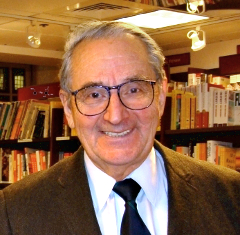
\includegraphics[width=\linewidth]{images/book3/corey.jpg}
\end{minipage}\hfill
\begin{minipage}[t]{0.76\linewidth}
\vspace{0pt}
रसायनज्ञ सदैव अपने लक्ष्यों से पीछे की ओर तर्क करते आए थे, परंतु इलायस जेम्स कोरी ने 1960 के दशक से
इस आदत को स्पष्ट नियमों में बदल दिया: \omterm{def:b2:retrosynthesis:disconnection}{विच्छेदन}, \omterm{def:b2:retrosynthesis:disconnection}{सिंथॉन}, पश्च-संश्लेषी तीर, और
उन्हें लागू करने वाले कंप्यूटर प्रोग्राम भी। कार्बनिक संश्लेषण के सिद्धांत और कार्यविधि के लिए उन्हें
1990 का रसायन का नोबेल पुरस्कार मिला। (छायाचित्र: ट्रुथकेम, CC0, विकिमीडिया कॉमन्स।)
\end{minipage}
\end{history}

\begin{safety}{\ghs[5mm]{GHS02}\,\ghs[5mm]{GHS03}\,\ghs[5mm]{GHS05}\,\ghs[5mm]{GHS06}\,\ghs[5mm]{GHS07}\,\ghs[5mm]{GHS08}}
ऑक्सैलिल क्लोराइड संक्षारक और विषैला है और जल से अभिक्रिया करके हाइड्रोजन क्लोराइड मुक्त करता है; स्वर्न
ऑक्सीकरण कार्बन मोनोऑक्साइड और दुर्गंधयुक्त डाइमेथिल सल्फ़ाइड मुक्त करता है, अतः इसे धूम-हुड में चलाया जाता है।
डेस--मार्टिन पीरियोडिनेन ऑक्सीकारक है और उसे गर्म नहीं करना चाहिए। जहाँ विकल्प उपलब्ध हो, वहाँ क्रोमियम(VI) अभिकर्मकों से
अब बचा जाता है।
% ledger: ghs:oxalyl-chloride, ghs:DMSO, ghs:DMP
\end{safety}

\section{अभ्यास}

\begin{exercise}[$\star$]\label{exo:b2:retrosynthesis:1}
हर ऐल्कोहॉल का एक कार्बोनिल यौगिक और एक ग्रीन्यार अभिकर्मक में \omterm{def:b2:retrosynthesis:disconnection}{विच्छेदन} कीजिए (हर संभावना दीजिए):
2-फ़ेनिलप्रोपेन-2-ऑल, पेंटेन-3-ऑल, 1-साइक्लोहेक्सिलएथेनॉल, 2-मेथिलब्यूटेन-2-ऑल, 1-फ़ेनिलएथेनॉल।
\end{exercise}

\begin{exercise}[$\star$]\label{exo:b2:retrosynthesis:2}
1-फ़ेनिलएथेनॉल के \ce{C-C} आबंध पर \omterm{def:b2:retrosynthesis:disconnection}{विच्छेदन} के लिए दोनों \omterm{def:b2:retrosynthesis:disconnection}{सिंथॉनों} के नाम बताइए, बताइए कि कौन-सा
दाता है, और हर एक का एक \omterm{def:b2:retrosynthesis:disconnection}{संश्लेषी तुल्य} दीजिए।
\end{exercise}

\begin{exercise}[$\star$]\label{exo:b2:retrosynthesis:3}
किसी पाँच-चरणीय मार्ग की चरण लब्धियाँ 90, 85, 80, 95 और 70~\% हैं। इसकी समग्र लब्धि परिकलित कीजिए।
\end{exercise}

\begin{exercise}[$\star$]\label{exo:b2:retrosynthesis:4}
एथिल 4-ऑक्सोपेंटेनोएट को 5-हाइड्रॉक्सीपेंटेन-2-ओन में बदलना है। किसी रक्षी
समूह के साथ मार्ग की योजना बनाइए, और बताइए कि वह क्यों आवश्यक है।
\end{exercise}

\begin{exercise}[$\star\star$]\label{exo:b2:retrosynthesis:5}
अधिकतम दो कार्बनों वाले यौगिकों से ब्यूटेन-1,3-डाइऑल का एक पश्च-संश्लेषण प्रस्तावित कीजिए, एक FGI और एक
द्वि-समूह \omterm{def:b2:retrosynthesis:disconnection}{विच्छेदन} के साथ।
\end{exercise}

\begin{exercise}[$\star\star$]\label{exo:b2:retrosynthesis:6}
\omterm{def:b2:frontier-orbitals:diels-alder}{डील्स--ऐल्डर अभिक्रिया} द्वारा 1-(साइक्लोहेक्स-3-ईन-1-इल)एथेन-1-ओन का \omterm{def:b2:retrosynthesis:disconnection}{विच्छेदन} कीजिए।
\end{exercise}

\begin{exercise}[$\star\star$]\label{exo:b2:retrosynthesis:7}
\omterm{def:b2:conjugate-additions:robinson}{रॉबिन्सन वलयन} द्वारा 4,4-डाइमेथिलसाइक्लोहेक्स-2-ईन-1-ओन का \omterm{def:b2:retrosynthesis:disconnection}{विच्छेदन} कीजिए।
\end{exercise}

\begin{exercise}[$\star\star$]\label{exo:b2:retrosynthesis:8}
1-फ़ेनिलब्यूटेन-1-ओन \omterm{def:b2:aromatic-substitution:friedel-crafts}{फ़्रीडेल--क्राफ़्ट्स ऐसिलन} द्वारा एक चरण में, या बेन्ज़ैल्डिहाइड से दो चरणों में बनाया जा सकता है।
दोनों मार्ग लिखिए और उनकी तुलना कीजिए।
\end{exercise}

\begin{exercise}[$\star\star$]\label{exo:b2:retrosynthesis:9}
हेक्सेन-1-ऑल से हेक्सेनल चाहिए। कौन-से अभिकर्मक इसे देते हैं, और कौन-सा इसके बजाय हेक्सेनोइक अम्ल
देगा? समझाइए।
\end{exercise}

\begin{exercise}[$\star\star\star$]\label{exo:b2:retrosynthesis:10}
4-ऐमीनोब्यूटेन-1-ऑल में ऐमीन को एक चरण में पहले किसी \omterm{def:b2:acyl-substitution:derivative}{ऐसिल क्लोराइड} से अभिक्रिया करनी है, और ऐल्कोहॉल को
बाद में किसी अन्य से। रक्षी समूहों का एक लांबिक युग्म और अनुक्रम प्रस्तावित कीजिए।
\end{exercise}

\begin{exercise}[$\star\star\star$]\label{exo:b2:retrosynthesis:11}
एथिल 3-ऑक्सोब्यूटेनोएट से हेक्सेन-2,5-डाइओन, एक 1,4-डाइकार्बोनिल यौगिक, का संश्लेषण प्रस्तावित कीजिए।
\end{exercise}

\begin{exercise}[$\star\star\star$]\label{exo:b2:retrosynthesis:12}
6-मेथिलहेप्ट-5-ईन-2-ओन, \ce{(CH3)2C=CHCH2CH2COCH3}, एक सुगंध मध्यवर्ती है। एथिल 3-ऑक्सोब्यूटेनोएट और
एक हैलाइड से पूरी योजना प्रस्तावित कीजिए: पश्च-संश्लेषण, आगे का मार्ग, और वह चरण जो
एस्टर को हटाता है।
\end{exercise}

\section{समस्या: रसभरी कीटोन}

\begin{problem}[{सप्ताहांत समस्या --- किसी सुवास यौगिक का पश्च-संश्लेषण, फ़ीनॉल और उसका
रक्षण किया जाए या नहीं, पैलेडियम विकल्प, और मार्गों का मूल्यांकन}]
\label{pb:b2:retrosynthesis:1}
रसभरी कीटोन, 4-(4-हाइड्रॉक्सीफ़ेनिल)ब्यूटेन-2-ओन, रसभरी और अन्य फलों में पाया जाता है और
सुवासक के रूप में और इत्र-निर्माण में प्रयुक्त होता है। अभ्यास के आँकड़े: \omterm{def:b2:enolates-aldol:aldol}{ऐल्डोल} मार्ग की चरण लब्धियाँ, 85~\% (संघनन)
और 92~\% (हाइड्रोजनन)। मोलर द्रव्यमान (\unit{g/mol}): C 12.011, H 1.008, O 15.999, N 14.007,
I 126.90। फ़ीनॉल का $\mathrm pK_a$ 9.99 है।
% ledger: use:raspberry-ketone, aw:C, aw:H, aw:O, aw:N, aw:I, pka:phenol, ghs:raspberry-ketone, ghs:4-iodophenol, ghs:MVK

\medskip
\noindent\textbf{भाग I --- पश्च-संश्लेषण।}
\begin{enumerate}
  \item लक्ष्य खींचिए और उसके क्रियात्मक समूहों के नाम बताइए।
  \item कौन-सा FGI \ce{ArCH2CH2CO} इकाई को ज्ञात \omterm{def:b2:retrosynthesis:disconnection}{विच्छेदन} वाले पैटर्न में बदलता है?
  \item प्राप्त असंतृप्त कीटोन उसकी ज्यामिति सहित लिखिए।
  \item इसमें कौन-सा द्वि-समूह पैटर्न है, और कौन-सी अभिक्रिया इसे बनाती है?
  \item दोनों आरंभिक पदार्थों के नाम बताइए।
  \item यह संकर \omterm{def:b2:enolates-aldol:aldol}{ऐल्डोल} एक मुख्य उत्पाद क्यों देता है?
  \item परिस्थितियों के साथ दो चरणों में आगे का मार्ग लिखिए।
\end{enumerate}

\medskip
\noindent\textbf{भाग II --- फ़ीनॉल।}
\begin{enumerate}[resume]
  \item जलीय सोडियम हाइड्रॉक्साइड में 4-हाइड्रॉक्सीबेन्ज़ैल्डिहाइड किस रूप में उपस्थित है?
        $\mathrm pK_a$ का उपयोग कीजिए।
  \item वह रूप ऐल्डिहाइड की इलेक्ट्रॉनरागिता को कैसे बदलता है?
  \item यदि फ़ीनॉल रक्षित होता, तो दूसरा चरण कौन-सा समूह मुफ़्त में हटा देता? समझाइए।
  \item उस रक्षण के साथ मार्ग के चरण गिनिए।
  \item क्या हाइड्रोजनन में बेन्ज़ीन वलय को ख़तरा है?
  \item रक्षण करें या नहीं? निष्कर्ष निकालिए।
\end{enumerate}

\medskip
\noindent\textbf{भाग III --- पैलेडियम विकल्प।}
\begin{enumerate}[resume]
  \item असंतृप्त कीटोन का वलय और शृंखला के बीच के आबंध पर \omterm{def:b2:retrosynthesis:disconnection}{विच्छेदन} कीजिए: कौन-से हेक
        भागीदार?
  \item क्षारक के रूप में ट्राइएथिलऐमीन के साथ हेक अभिक्रिया लिखिए।
  \item ऐरिल समूह ब्यूट-3-ईन-2-ओन के किस कार्बन पर पहुँचता है, और क्यों?
  \item \omterm{def:b2:catalytic-cycles:cycle}{उत्प्रेरकी चक्र} के चरणों के नाम बताइए।
  \item ट्राइएथिलऐमीन को गिनते हुए हेक चरण की परमाणु मितव्ययिता परिकलित कीजिए।
  \item \omterm{def:b2:enolates-aldol:aldol}{ऐल्डोल संघनन} की परमाणु मितव्ययिता परिकलित कीजिए।
\end{enumerate}

\medskip
\noindent\textbf{भाग IV --- मार्गों का मूल्यांकन।}
\begin{enumerate}[resume]
  \item हाइड्रोजनन की परमाणु मितव्ययिता क्या है?
  \item \omterm{def:b2:enolates-aldol:aldol}{ऐल्डोल} मार्ग की समग्र परमाणु मितव्ययिता परिकलित कीजिए।
  \item हाइड्रोजनन किस द्वि-आबंध का अपचयन करता है, और कीटोन क्यों बच जाता है?
  \item दोनों मार्गों के अभिकर्मकों की क़ीमत और ख़तरे के लिए तुलना कीजिए।
  \item आप कौन-सा मार्ग चुनेंगे?
  \item 90~\% पर एक तीसरा चरण समग्र लब्धि पर क्या प्रभाव डालता?
  \item दो-चरणीय \omterm{def:b2:enolates-aldol:aldol}{ऐल्डोल} मार्ग की समग्र लब्धि बताइए।
\end{enumerate}
\end{problem}
